\documentclass[a4paper,11pt,dvipdfmx]{ujarticle}
% パッケージ
\usepackage{graphicx}
\usepackage{url}
% レイアウト指定を記述したファイルの読み込み
\input{layout}

% タイトルと氏名を変更せよ.
\title{日本におけるデジタル化の状況}
\author{千野 琉斗}

\begin{document}

\maketitle %ここにタイトルが入る

% ここから本文
\section{デジタル競争力ランキング}
% を使う

国際経営開発研究所(IMD)の調査\cite{imd}によると、日本のデジタル競争力のランキングは図\ref{fig:ランキング}に示すよ
うに、調査対象の64カ国中、総合で28位、技術分野で30位となっている。
\begin{figure}[htbp]
    \centering
    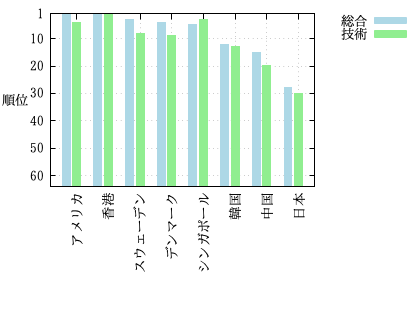
\includegraphics[width=0.7\linewidth]{fig41.png}
    \caption{情報通信機器の世帯保有率}\label{fig:ランキング}
\end{figure}
%  参考文献の参照: \cite{}
%  図番号の参照: \ref{}
% を使う
% 文献データベースのキーワードは oecd と imd
% になっている.
\newpage



% 図の挿入
% \includegraphics{}
% を
% \begin{figure}[htbp]
% \end{figure}
% で囲み
% \caption{}
% で図のタイトルを入れる.
% \label{}
% を使って図番号が参照できるようにする
% また,
% \centering
% で図が中央に来るようにする

% ーーー
% 節見出し(2)
\section{ブロードバンド整備状況}
OECDによるブロードバンド回線の普及に関する調査\cite{oecd}によると、表\ref{tbl:利用状況}に示すように、日本における 100人あたりのモバイルブロードバンドの加入者数は190.5で、第1位になっている。2位はエストニア
で、3位米国と続く。

\begin{table}[htbp]
    \centering
    \caption{:モバイルブロードバンドの加入者数(100人あたり)}
    \label{tbl:利用状況}

    \begin{tabular}{|l|l||r|}\hline
        順位 & 国名 & 加入者数 \\
        \hline
        1位 & 日本 & 190.5 \\
        \hline
        2位 & エストニア & 179.9 \\
        \hline
        3位 & 米国 & 169.0 \\
        \hline
        4位 & フィンランド & 157.0 \\
        \hline
        5位 & デンマーク & 141.7 \\
        \hline
        6位 & ラトビア & 141.6 \\
        \hline 
        7位 & イスラエル & 139.9 \\
        \hline
        8位 & オランダ & 133.7 \\
        \hline
        9位 & ポーランド & 131.3 \\
        \hline
        10位 & スウェーデン & 127.2 \\
        \hline
    \end{tabular}
\end{table}
% 本文(2)

% 表の挿入
% \begin{tabular}
% \end{tabular}    
% による表の記述を 
% \begin{table}[htbp]
% \end{table}
% で囲み
% \caption{}
% で表のタイトルを入れる.
% \label{}
% を使って表番号が参照できるようにする
% また,
% \centering
% で表が中央に来るようにする

% ーーー
% 見出し(3)
\section{考察}
\begin{itemize}
    \item 日本はハード面では優れているが、ソフト面で他国より劣っているのが競争力の低さの原因だと感じた。
    \item 世界のデジタル化のスピードに遅れないよう、継続的な政策と社会全体の意識改革が必要である。
\end{itemize}
% \end{itemize}
% を使って箇条書きで記述する

% ここに参考文献が入る
%
\bibliographystyle{junsrt}
\bibliography{exercise.bib}

\end{document}